\documentclass[
presentation, % always use this
%handout % use this to have 4 slides per page and space for notes at the side
]{beamer}
\usepackage[utf8]{inputenc}


\usetheme[
%color=white,	% blue (not well supported) or white
%titleimage,    % use TUM flags on title slide (experimental)
%conference,    % if present, logos appear only on title page (not CI compliant)
%rcslogo,	% include RCS logo in header (ignored if nonci is present)
%headfootlines,  % if present, separate header and footer by line (not CI compliant)
nonci,	        % if present, then deviate from  TUM-CI (obviously, not CI compliant)
%tumfont   % if present, use TUM Neue Helvetica (must be installed)
]{rcs}


\title[A TUM RCS theme for \LaTeX~beamer class]{A TUM RCS theme for \LaTeX~beamer class}
\subtitle{Better presentations}
\author[Becker]{%
  Martin~Becker\inst{1} \and
  Martin~Becker\inst{2}}
\institute[RCS]{
  \inst{1}%
  Real-Time Computer Systems (RCS)\\
  Technische Universität München
  \and
  \inst{2}%
  Real-Time Computer Systems (RCS)\\
  Technische Universität München}
\date{\today}
\subject{Beamer Theme}

\begin{document}

\begin{frame}[plain]
\maketitle
\end{frame}

\frame{\frametitle{Table of contents}\tableofcontents}

\section{Introduction}
\subsection{About}
\begin{frame}[fragile]
\frametitle{About}

\begin{itemize}
\item a \LaTeX~beamer theme according to TUM CI (2016)
  \begin{itemize}
  \item colors, fonts, arrangements, ... all compliant!
  \end{itemize}
\item this presentation is shipped as \texttt{example.tex}
\item just run it through \texttt{pdflatex}
\item only for \alert{pdflatex}, \alert{latex} not supported 
  \begin{itemize}
  \item only because TUM fonts are not available then
  \end{itemize}
\end{itemize}
\end{frame}

\section{Installation}
\begin{frame}[fragile]
  \frametitle{Install Notes}
  \begin{itemize}
  \item install this template following README
  \item optionally, install TUM fonts first:
    \begin{itemize}
    \item grab TUM's Latex brief class \href{http://portal.mytum.de/corporatedesign/download/index_html/LaTeX_Vorlagen}{\textit{from mytum.de}}:\\
      {\tiny\texttt{http://portal.mytum.de/corporatedesign/download/LaTeX\_Vorlagen/tum-texmf-2.0.85.tgz}}\\
      {\tiny\texttt{http://portal.mytum.de/corporatedesign/download/LaTeX\_Vorlagen/tum-texmf-2.0.85.zip}}
    \item and follow their install instructions
    \end{itemize}
  \item then enable the fonts with the \texttt{tumfont} option
  \end{itemize}
\end{frame}


\section{Usage}
\begin{frame}[fragile]
  \frametitle{Using the theme} 
  \framesubtitle{What options do I have?}
  General usage: 
    \begin{lstlisting}
\usetheme[option1,option2,...]{rcs}
    \end{lstlisting}
  With the following options:
  \begin{itemize}
  \item default is a CI-compliant scheme
  \item more space (move slide title to top of frame), use \texttt{nonci}
  \item to switch the TUM logo for the RCS logo use \texttt{rcslogo}
  \item To get a title page with background image use \texttt{titleimage}
  \item To add header/footer separation lines, use \texttt{headfootlines}
  \item Suggested options (not TUM CI compliant)
    \lstset{language=TeX}
    \begin{lstlisting}
\usetheme[nonci]{rcs}
    \end{lstlisting}        
  \item \alert{Last but not least}, use this to get a handout version with 4 slides per page: \texttt{\textbackslash documentclass[handout]\{beamer\}}
  \end{itemize}
\end{frame}

\begin{frame}[fragile]
  \frametitle{Using the theme (2)} 
  \framesubtitle{Can I change placement of logos?}
  \begin{itemize}
  \item If you don't like the CI-compliant slide layout, there is an alternative that uses smaller fonts and places the headings above headsepline:
    \begin{lstlisting}
\usetheme[nonci]{rcs}
    \end{lstlisting}
  \item For conferences, there is a switch to disable all logos except on the title page:
    \begin{lstlisting}
\usetheme[conference]{rcs}
    \end{lstlisting}
  \item \alert{above two options cannot be used together}
  \end{itemize}
\end{frame}

\begin{frame}[fragile]
  \frametitle{Using the theme (3)} 
  \framesubtitle{Changing Fonts}
  \begin{itemize}
  \item by default, this template uses lmodern fonts (sans serif)
  \item if you want the TUM font or you get serif fonts, then use
    \begin{lstlisting}
\usetheme[tumfont]{rcs}
    \end{lstlisting}
  \end{itemize}
\end{frame}


\section{Examples}
\subsection{Titles and stuff}
\frame{ 
Without title something is missing. 
 }

\frame{\frametitle{unnumbered lists}
This is \alert{something important} that needs to be stressed. And \emph{this is emphasized}.
}


\subsection{Lists I}
\frame{\frametitle{unnumbered lists}
\begin{itemize}
\item Introduction to  \LaTeX  
\item Course 2
\item Termpapers and presentations with \LaTeX 
\item Beamer class
\end{itemize} 
}

\subsection{Blocks}
\frame{\frametitle{block}
\begin{block}{This is a Block}
      This is important information
   \end{block}
}
\frame{\frametitle{example block}
   \begin{exampleblock}{This is an Example block}
   This is an example 
   \end{exampleblock}

}
\frame{\frametitle{alert block}
   \begin{alertblock}{This is an Alert block}
   This is an important alert
   \end{alertblock}
}

\subsection{Source Code}
\begin{frame}[fragile]
\frametitle{code blocks}
Beautified and highlighted in CI colors as well ...
    \lstset{language=C}
    \begin{lstlisting}
printf("Hello World!\n");
if (1 == 1) {
  int a = 0;
} else {
  /* get out */
  return false;
}
    \end{lstlisting}
\end{frame}

\subsection{Lists II}
\frame{\frametitle{numbered lists}
\begin{enumerate}
\item Introduction to  \LaTeX  
\item Course 2
\item Termpapers and presentations with \LaTeX 
\item Beamer class
\end{enumerate}
}
\frame{\frametitle{numbered lists with pause}
\begin{enumerate}
\item Introduction to  \LaTeX \pause 
\item<1-> Course 2 \pause 
\item<2-> Termpapers and presentations with \LaTeX \pause 
\item<3-> Beamer class
\end{enumerate}
}

\subsection{Images}
\frame{\frametitle{Images}
 
  \begin{columns}[t]
    \begin{column}{.4\textwidth}
      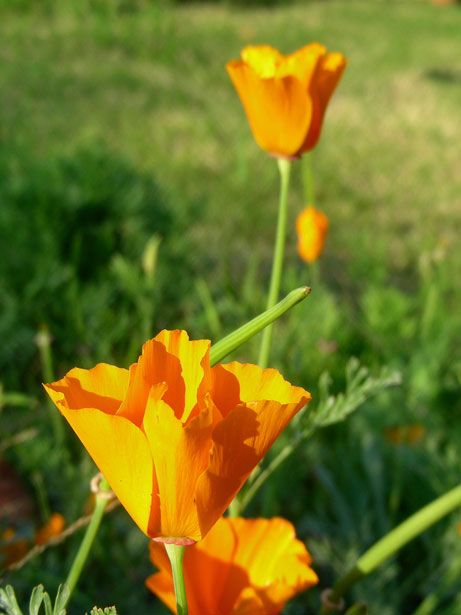
\includegraphics[height=.7\textheight]{mohn.jpg}
    \end{column}
    \begin{column}{.4\textwidth}
      \begin{itemize}
      \item some text goes here
      \item this is a flower
      \end{itemize}
    \end{column}
  \end{columns}
}


\end{document}

%%% Local Variables: 
%%% mode: pdflatex
%%% TeX-master: t
%%% End: 
